% ============================================================
%  KubeRift — Complete User Manual
%  Engine : XeLaTeX
%  Fonts  : EB Garamond (body) · IBM Plex Sans (headings) · IBM Plex Mono (code)
% ============================================================
\documentclass[11pt, a4paper, twoside]{article}

% ── Core XeLaTeX / font machinery ────────────────────────────
\usepackage{fontspec}

% Body — Cormorant Garamond (proper OTF with separate weight files)
\setmainfont{Cormorant Garamond}[
  Ligatures     = TeX,
]

% Headings — IBM Plex Sans
\setsansfont{IBM Plex Sans}[
  Scale         = MatchLowercase,
]

% Monospace — IBM Plex Mono (tight, technical)
\setmonofont{IBM Plex Mono}[
  Scale         = 0.87,
]

% ── Page geometry ─────────────────────────────────────────────
\usepackage[
  a4paper,
  top=22mm, bottom=24mm,
  inner=22mm, outer=18mm,
  headheight=22pt,
  headsep=8mm,
  footskip=12mm,
]{geometry}

% ── Micro-typography ─────────────────────────────────────────
\usepackage[final, protrusion=true]{microtype}

% ── Colors ───────────────────────────────────────────────────
\usepackage{xcolor}
\definecolor{KRblue}{HTML}{1A3A5C}      % deep navy — brand primary
\definecolor{KRteal}{HTML}{0A7B8A}      % teal — accent / headings
\definecolor{KRrust}{HTML}{B04A2F}      % rust orange — code accent
\definecolor{KRgray}{HTML}{5C6370}      % neutral gray
\definecolor{KRlight}{HTML}{F4F7FA}     % very light blue-gray — boxes
\definecolor{KRborder}{HTML}{C5D8EC}    % soft border
\definecolor{codegreen}{HTML}{3D7A3D}
\definecolor{codegray}{HTML}{888888}
\definecolor{codepurple}{HTML}{6B3FA0}

% ── Graphics & TikZ ──────────────────────────────────────────
\usepackage{tikz}
\usetikzlibrary{arrows.meta, shapes.geometric, positioning, fit, backgrounds, calc}

% ── Headers & footers ────────────────────────────────────────
\usepackage{fancyhdr}
\pagestyle{fancy}
\fancyhf{}
\renewcommand{\headrulewidth}{0.4pt}
\renewcommand{\headrule}{\hbox to\headwidth{\color{KRteal}\leaders\hrule height\headrulewidth\hfill}}
\fancyhead[LE]{\small\sffamily\color{KRgray}\textit{KubeRift User Manual}}
\fancyhead[RO]{\small\sffamily\color{KRgray}\nouppercase{\leftmark}}
\fancyfoot[C]{\small\sffamily\color{KRgray}\thepage}
\fancypagestyle{plain}{%
  \fancyhf{}
  \renewcommand{\headrulewidth}{0pt}
  \fancyfoot[C]{\small\sffamily\color{KRgray}\thepage}
}

% ── Section styling ──────────────────────────────────────────
\usepackage{titlesec}
\titleformat{\section}
  {\sffamily\large\bfseries\color{KRblue}}
  {\thesection}{0.8em}{}
  [\vspace{-2pt}{\color{KRteal}\titlerule[0.6pt]}]
\titleformat{\subsection}
  {\sffamily\normalsize\bfseries\color{KRteal}}
  {\thesubsection}{0.7em}{}
\titleformat{\subsubsection}
  {\sffamily\small\bfseries\color{KRgray}}
  {}{0em}{}

\titlespacing*{\section}{0pt}{1.4ex plus .4ex}{0.5ex plus .2ex}
\titlespacing*{\subsection}{0pt}{1ex plus .3ex}{0.3ex}
\titlespacing*{\subsubsection}{0pt}{0.8ex}{0.2ex}

% ── Paragraph style ──────────────────────────────────────────
\usepackage{parskip}
\setlength{\parskip}{4pt plus 1pt}
\setlength{\parindent}{0pt}
\setlength{\emergencystretch}{3em}   % allow extra stretch to avoid overfull hboxes

% ── Lists ────────────────────────────────────────────────────
\usepackage{enumitem}
\setlist[itemize]{leftmargin=1.2em, itemsep=1pt, parsep=0pt, topsep=3pt}
\setlist[enumerate]{leftmargin=1.4em, itemsep=1pt, parsep=0pt, topsep=3pt}

% ── Tables ───────────────────────────────────────────────────
\usepackage{booktabs}
\usepackage{array}
\usepackage{longtable}
\newcolumntype{L}[1]{>{\raggedright\arraybackslash}p{#1}}
\newcolumntype{C}[1]{>{\centering\arraybackslash}p{#1}}

% ── Boxes / callouts ─────────────────────────────────────────
\usepackage{tcolorbox}
\tcbuselibrary{skins, breakable, listings}

\newtcolorbox{notebox}[1][]{
  enhanced, breakable,
  colback=KRlight, colframe=KRborder,
  left=4pt, right=4pt, top=3pt, bottom=3pt,
  fonttitle=\sffamily\small\bfseries\color{KRblue},
  title={#1},
  coltitle=KRblue,
  attach boxed title to top left={yshift=-2mm, xshift=4mm},
  boxed title style={colback=KRlight, colframe=KRborder},
  arc=3pt,
}

\newtcolorbox{warningbox}{
  enhanced, breakable,
  colback=KRrust!7, colframe=KRrust!50,
  left=4pt, right=4pt, top=3pt, bottom=3pt,
  arc=3pt,
}

\newtcolorbox{keybox}{
  enhanced,
  colback=KRblue!8, colframe=KRblue!30,
  left=4pt, right=4pt, top=2pt, bottom=2pt,
  arc=2pt,
  fontupper=\small\sffamily,
}

% ── Code listings ─────────────────────────────────────────────
\usepackage{listings}

% Define Rust as a custom language (not built into listings)
\lstdefinelanguage{Rust}{
  keywords={pub, fn, struct, impl, let, mut, async, await, use, match,
            if, else, return, for, while, loop, break, continue, in,
            where, type, trait, enum, mod, crate, super, self, true, false,
            const, static, move, ref, Box, Arc, Option, Result, Some, None,
            Ok, Err, String, Vec, HashMap, tokio, spawn},
  sensitive=true,
  comment=[l]{//},
  morecomment=[s]{/*}{*/},
  morestring=[b]",
  morestring=[b]',
}

\lstdefinestyle{rust}{
  language=Rust,
  basicstyle=\small\ttfamily\color{KRblue!80!black},
  keywordstyle=\bfseries\color{codepurple},
  commentstyle=\itshape\color{codegray},
  stringstyle=\color{KRrust},
  identifierstyle=\color{KRblue},
  backgroundcolor=\color{KRlight},
  frame=single, framerule=0.4pt,
  rulecolor=\color{KRborder},
  breaklines=true, breakatwhitespace=true,
  showstringspaces=false,
  numbers=none,
  xleftmargin=6pt, xrightmargin=6pt,
  aboveskip=4pt, belowskip=4pt,
  tabsize=4,
  morekeywords={pub, fn, struct, impl, let, mut, async, await, use, match, Arc, Option, Result},
}
\lstdefinestyle{shell}{
  basicstyle=\small\ttfamily\color{KRblue!90},
  backgroundcolor=\color{KRblue!5},
  frame=single, framerule=0.4pt,
  rulecolor=\color{KRborder},
  breaklines=true,
  showstringspaces=false,
  xleftmargin=6pt, xrightmargin=6pt,
  aboveskip=4pt, belowskip=4pt,
}
\lstset{style=shell}

% ── Hyperlinks ────────────────────────────────────────────────
\usepackage{hyperref}
\hypersetup{
  colorlinks=true,
  linkcolor=KRteal,
  urlcolor=KRteal,
  citecolor=KRteal,
  pdftitle={KubeRift User Manual},
  pdfauthor={Syed Azeez},
  pdfsubject={Kubernetes TUI Operations Platform},
}

% ── Utilities ────────────────────────────────────────────────
\usepackage{multicol}
\usepackage{graphicx}
\usepackage{eso-pic}   % for background on title page

% ── Keyboard key macro ────────────────────────────────────────
\newcommand{\kbd}[1]{%
  \tikz[baseline=(k.base)]{
    \node[draw=KRgray!60, rounded corners=2pt,
          inner xsep=2.5pt, inner ysep=1.5pt,
          fill=KRlight, font=\small\ttfamily] (k) {#1};
  }%
}

% ── Inline code ───────────────────────────────────────────────
\newcommand{\code}[1]{\texttt{\color{KRrust}#1}}

% ── Chapter-like block for opening pages ──────────────────────
\newcommand{\chapteropen}[2]{%
  \clearpage
  \begin{tikzpicture}[remember picture, overlay]
    \fill[KRblue] (current page.north west)
      rectangle ([yshift=-28mm]current page.north east);
    \node[anchor=west, text=white, font=\sffamily\Large\bfseries]
      at ([xshift=22mm, yshift=-14mm]current page.north west) {#1};
    \node[anchor=west, text=KRborder, font=\sffamily\small]
      at ([xshift=22mm, yshift=-22mm]current page.north west) {#2};
  \end{tikzpicture}
  \vspace*{12mm}
}

% ============================================================
\begin{document}
% ============================================================

% ── TITLE PAGE ───────────────────────────────────────────────
\begin{titlepage}
  \begin{tikzpicture}[remember picture, overlay]
    % full-bleed navy top band
    \fill[KRblue]
      (current page.north west)
      rectangle ([yshift=-120mm]current page.north east);
    % teal diagonal accent
    \fill[KRteal!80!black]
      ([yshift=-110mm]current page.north west) --
      ([yshift=-120mm]current page.north west) --
      ([yshift=-120mm]current page.north east) --
      ([yshift=-100mm]current page.north east) -- cycle;
    % bottom stripe
    \fill[KRteal!30!white, opacity=0.18]
      (current page.south west)
      rectangle ([yshift=18mm]current page.south east);
  \end{tikzpicture}

  \vspace*{30mm}

  % Logo / wordmark block
  {\color{white}\sffamily
    \hspace*{22mm}%
    {\fontsize{42}{46}\selectfont\bfseries KubeRift}

    \vspace{3mm}
    \hspace*{22mm}%
    {\large\color{KRborder} Fuzzy-First Kubernetes Operations Platform}
  }

  \vspace{40mm}

  % Subtitle box
  \hspace*{22mm}%
  \begin{minipage}{0.74\textwidth}
    \begin{tcolorbox}[
      colback=KRlight, colframe=KRteal,
      arc=4pt, left=8pt, right=8pt, top=6pt, bottom=6pt,
    ]
      \sffamily\small
      A complete reference for installing, operating, and extending KubeRift ---
      the terminal-native Kubernetes navigator written in Rust.
      Covers architecture, all keyboard actions, multi-cluster workflows,
      security model, and the open-source story of how a fuzzy-finder library
      became the foundation of a Kubernetes operations platform.
    \end{tcolorbox}
  \end{minipage}

  \vfill

  % Metadata grid
  \hspace*{22mm}%
  \begin{minipage}{0.74\textwidth}
    \small\sffamily\color{KRgray}
    \begin{tabular}{@{}l l}
      \textbf{Version}   & 0.1.2 \\[1pt]
      \textbf{Binary}    & \code{kf} \\[1pt]
      \textbf{Source}    & \href{https://github.com/syedazeez337/kuberift}{github.com/syedazeez337/kuberift} \\[1pt]
      \textbf{Crate}     & \href{https://crates.io/crates/kuberift}{crates.io/crates/kuberift} \\[1pt]
      \textbf{License}   & MIT \\[1pt]
      \textbf{Date}      & March 2026 \\
    \end{tabular}
  \end{minipage}

  \vspace{10mm}
\end{titlepage}

% ── TABLE OF CONTENTS ────────────────────────────────────────
\tableofcontents
\clearpage

% ============================================================
%  SECTION 1 — THE SKIM STORY
% ============================================================
\chapteropen{The Skim Insight}{How a fuzzy-finder library became the load-bearing wall of a Kubernetes platform}

\section{The Skim Insight: Architecture Born from a Library}
\markboth{The Skim Insight}{}

\subsection{The Problem Space}

\begin{sloppypar}
Every Kubernetes practitioner eventually arrives at the same frustration: \texttt{kubectl get pods -{}-all-namespaces} produces a wall of text, \texttt{kubectl describe} requires knowing the exact resource name, and switching between resource types means retyping commands. Existing tools like k9s take a ``modal'' approach---navigate menus, select a resource type, then a namespace, then an item---borrowed from graphical file managers.
\end{sloppypar}

KubeRift was conceived around a different premise: \emph{what if the search box is the interface?} Type fragments of a pod name, a namespace, a status --- the list filters instantly. No modes, no menus, no hierarchy to navigate. Just a fuzzy query and a live list.

That idea pointed immediately to a fuzzy-finder. But which one, and how?

\subsection{Discovering Skim as a Library}

The first prototype used \textbf{fzf} --- the ubiquitous Go binary --- through a subprocess pipe. It worked but felt architecturally wrong: items had to be serialized to plain text strings, sent through a pipe, and the selection had to be parsed back. Colors required ANSI escapes baked into strings. Preview required a shell command string. Multi-select results came back as newline-delimited text. Every richness in the Rust data model was lost at the pipe boundary and had to be laboriously reconstructed.

The pivotal discovery came from reading the README of \textbf{skim} (\href{https://crates.io/crates/skim}{crates.io/crates/skim}), a fuzzy finder written in Rust and MIT-licensed. Its README opens with a distinction invisible in most tools:

\begin{notebox}[Note from the skim README]
  \small\itshape
  ``Skim can be used as a library in your Rust project. The library allows you to embed
  the fuzzy-finder TUI directly in your binary and receive typed, structured results
  back --- no subprocess, no pipe, no string serialization.''
\end{notebox}

This changed everything. Not a subprocess to spawn but a \emph{trait to implement.}

\subsection{The \texttt{SkimItem} Trait as Architectural Foundation}

The \code{SkimItem} trait has four methods. Each one became a design decision that propagated through every layer of KubeRift:

\begin{lstlisting}[style=rust]
pub trait SkimItem: Send + Sync + 'static {
    fn text(&self) -> Cow<str>;          // what skim fuzzy-matches against
    fn display(&self, ctx: DisplayContext) -> AnsiString; // colored list row
    fn preview(&self, ctx: PreviewContext) -> ItemPreview; // right-hand pane
    fn output(&self) -> Cow<str>;        // machine-parseable selection result
}
\end{lstlisting}

\textbf{\code{text()}} determined the search schema. To make a pod searchable by name, namespace, kind, status, and age simultaneously, all those fields had to be concatenated into a single string. This forced the design of \code{K8sItem} as a self-contained value type carrying all metadata.

\textbf{\code{display()}} established the visual contract. Because skim calls this on every render frame, the color-coding logic (red for critical, yellow for warning, green for healthy) had to be fast and allocation-minimal. The \code{StatusHealth} enum and its \code{classify()} function emerged directly from this requirement.

\textbf{\code{preview()}} revealed the threading model. Skim calls \code{preview()} from a \emph{background thread} whenever the cursor moves. This is a blocking call --- perfect for synchronous \code{kubectl} invocation. But supporting three preview modes (describe / yaml / logs) meant the preview function needed to read external state. The solution: a tiny file in \code{\$XDG\_RUNTIME\_DIR/<pid>/preview-mode} containing a single digit. The \code{ctrl-p} binding writes a new digit to that file and signals skim to refresh. Clean, race-free, zero shared memory.

\textbf{\code{output()}} defined the action dispatch protocol. The string \code{"pod/production/api-server/my-context"} became the canonical identifier threaded through every action function. The double-dash separator (\code{--}) before resource names in every kubectl invocation is a direct consequence of needing to reconstruct safe command lines from this identifier.

\subsection{The Channel as the System's Spine}

The second architectural insight was skim's \code{SkimItemSender}/\code{SkimItemReceiver} channel pair:

\begin{lstlisting}[style=rust]
let (tx, rx): (SkimItemSender, SkimItemReceiver) = unbounded();

tokio::spawn(async move {
    // K8s watcher sends items as they arrive from the API
    while let Some(event) = watcher.next().await {
        tx.send(Arc::new(K8sItem::from(event))).ok();
    }
});

// Skim consumes from rx -- items appear as the cluster streams them
let output = Skim::run_with(&options, Some(rx));
\end{lstlisting}

This is a \textbf{multi-producer, single-consumer} pattern. For multi-cluster mode, it becomes \emph{multi-producer}: one tokio task per kubeconfig context, all sending into the same channel, all items converging in a single skim session. The architecture handles one cluster and twenty clusters identically --- the channel is the only integration point.

\subsection{The Key Dispatch Pattern}

Skim's \code{SkimOutput} returns a \code{final\_key} field --- whichever key ended the session. KubeRift registers every action key with the \code{accept} binding rather than \code{execute}. This means control always returns to Rust:

\begin{lstlisting}[style=rust]
match output.final_key {
    Key::Enter     => action_describe(&items).await?,
    Key::Ctrl('l') => action_logs(&items).await?,
    Key::Ctrl('e') => action_exec(&items[0]).await?,
    Key::Ctrl('d') => action_delete(&items).await?,
    Key::Ctrl('f') => action_portforward(&items[0]).await?,
    Key::Ctrl('r') => action_rollout_restart(&items).await?,
    Key::Ctrl('y') => action_yaml(&items).await?,
    Key::Ctrl('x') => { /* context switch, relaunch */ }
    _ => {}
}
\end{lstlisting}

After every action, skim relaunches with a fresh channel but the same configuration. The user sees the live cluster list again, uninterrupted. This loop-after-action design means KubeRift feels more like a shell than an application --- you run commands, you return to the prompt.

\begin{keybox}
  \textbf{The founding insight in one sentence:} Skim's \code{SkimItem} trait, its MPSC item channel, and its \code{final\_key} dispatch pattern collectively determined KubeRift's data model, threading architecture, preview mechanism, and action system --- before a single line of Kubernetes code was written.
\end{keybox}

% ============================================================
%  SECTION 2 — ARCHITECTURE
% ============================================================
\clearpage
\section{System Architecture}
\markboth{System Architecture}{}

KubeRift is a single Rust binary structured in three layers that communicate through well-defined interfaces.

\subsection{Layer Map}

\begin{center}
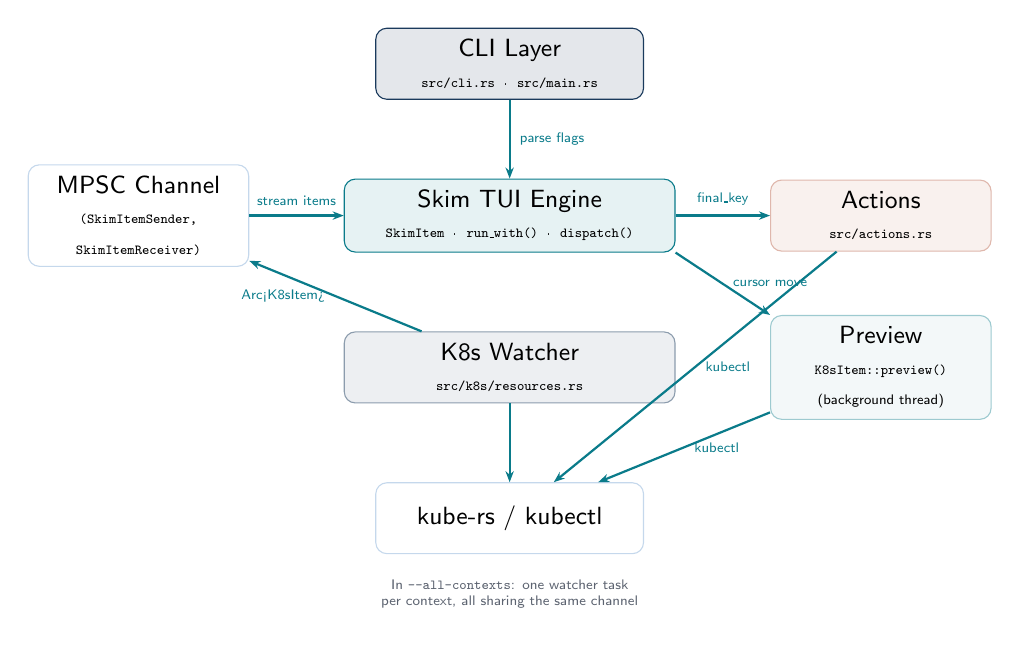
\begin{tikzpicture}[
  node distance=5mm and 8mm,
  box/.style={
    draw=KRblue!40, rounded corners=4pt,
    fill=KRlight, minimum width=34mm, minimum height=9mm,
    font=\small\sffamily, align=center, inner sep=4pt
  },
  arrow/.style={-{Stealth[length=4pt]}, thick, color=KRteal},
  label/.style={font=\tiny\sffamily\color{KRgray}, midway},
]

% Layer 1 — Entry
\node[box, fill=KRblue!12, draw=KRblue] (cli) {CLI Layer\\\tiny\texttt{src/cli.rs · src/main.rs}};

% Layer 2 — TUI Engine (center)
\node[box, fill=KRteal!10, draw=KRteal, minimum width=42mm, below=10mm of cli] (skim)
  {Skim TUI Engine\\\tiny\texttt{SkimItem · run\_with() · dispatch()}};

% Channels
\node[box, fill=white, draw=KRborder, left=12mm of skim, minimum width=28mm]
  (chan) {MPSC Channel\\\tiny\texttt{(SkimItemSender,}\\\tiny\texttt{SkimItemReceiver)}};

% Layer 3 — K8s
\node[box, fill=KRblue!8, draw=KRblue!50, below=10mm of skim, minimum width=42mm]
  (watcher) {K8s Watcher\\\tiny\texttt{src/k8s/resources.rs}};

% Actions
\node[box, fill=KRrust!8, draw=KRrust!40, right=12mm of skim, minimum width=28mm]
  (actions) {Actions\\\tiny\texttt{src/actions.rs}};

% Preview
\node[box, fill=KRteal!5, draw=KRteal!40, right=12mm of watcher, minimum width=28mm]
  (preview) {Preview\\\tiny\texttt{K8sItem::preview()}\\\tiny(background thread)};

% kube-rs / kubectl
\node[box, fill=white, draw=KRborder, below=10mm of watcher]
  (kube) {kube-rs / kubectl};

% Arrows
\draw[arrow] (cli) -- node[right, label]{parse flags} (skim);
\draw[arrow] (chan) -- node[above, label]{stream items} (skim);
\draw[arrow] (watcher) -- node[left, label]{Arc<K8sItem>} (chan);
\draw[arrow] (watcher) -- (kube);
\draw[arrow] (skim) -- node[above, label]{final\_key} (actions);
\draw[arrow] (actions) -- node[right, label]{kubectl} (kube);
\draw[arrow] (skim.south east) -- node[right, label]{cursor move} (preview.north west);
\draw[arrow] (preview) -- node[right, label]{kubectl} (kube);

% Multi-cluster note
\node[font=\tiny\sffamily\color{KRgray}, below=2mm of kube, text width=42mm, align=center]
  {In \texttt{-{}-all-contexts}: one watcher task per context, all sharing the same channel};

\end{tikzpicture}
\end{center}

\subsection{Component Responsibilities}

\textbf{CLI Layer} (\code{src/cli.rs}, \code{src/main.rs})\quad Parses arguments via Clap, resolves the kubeconfig, determines single vs.\ multi-cluster mode, constructs the skim options (header text, keybinding strings, preview window placement), and drives the outer \code{loop \{ skim → dispatch → relaunch \}}.

\textbf{K8s Watcher} (\code{src/k8s/resources.rs}, \code{src/k8s/client.rs})\quad Uses \code{kube::runtime::watcher} to stream \texttt{Applied}/\texttt{Deleted} events for all thirteen resource kinds concurrently. A coordinator task collects the initial batch, sorts by health priority (unhealthy first), and flushes to the channel. Subsequent live events are forwarded immediately.

\textbf{Skim TUI Engine}\quad The embedded fuzzy-finder. Renders the list, handles keyboard input, calls \code{display()} on every frame and \code{preview()} on cursor movement. Returns a \code{SkimOutput} to Rust.

\textbf{Actions} (\code{src/actions.rs})\quad Pure functions that receive a slice of \code{Arc<K8sItem>} and shell out to \code{kubectl}. All commands use \code{--} before resource names (argument injection prevention). Dangerous operations include interactive confirmation.

\textbf{Preview Thread}\quad Skim's internal background thread calls \code{K8sItem::preview()}, which reads the mode file and runs \code{kubectl describe}, \code{kubectl get -o yaml}, or \code{kubectl logs}.

\subsection{Unhealthy-First Ordering}

Health classification drives sort priority:

\begin{center}
\small\sffamily
\begin{tabular}{@{}L{38mm} C{20mm} L{60mm}@{}}
\toprule
\textbf{Status examples} & \textbf{Priority} & \textbf{Display color} \\
\midrule
CrashLoopBackOff, OOMKilled, Error, ImagePullBackOff & 0 — Critical & \textcolor{red!70!black}{\textbf{Red}} \\
Pending, NotReady, Degraded (N/M), Terminating & 1 — Warning & \textcolor{orange!80!black}{\textbf{Yellow}} \\
Running, Ready, Bound, Active, Scheduled & 2 — Healthy & \textcolor{green!50!black}{\textbf{Green}} \\
\texttt{{[}DELETED{]}} & 1 — Unknown & \textcolor{gray}{\textbf{Dark gray}} \\
\bottomrule
\end{tabular}
\end{center}

Skim renders higher-indexed items at the \emph{top} of the list. The watcher sends critical items \emph{last} in the initial batch so they receive the highest indices and surface automatically without any filter.

% ============================================================
%  SECTION 3 — INSTALLATION & QUICK START
% ============================================================
\clearpage
\section{Installation \& First Run}
\markboth{Installation \& First Run}{}

\subsection{Install Methods}

\textbf{Cargo (all platforms):}
\begin{lstlisting}
cargo install kuberift
\end{lstlisting}

\textbf{Homebrew (macOS and Linux):}
\begin{lstlisting}
brew tap syedazeez337/kuberift
brew install kf
\end{lstlisting}

\textbf{Arch Linux (AUR):}
\begin{lstlisting}
yay -S kuberift          # or paru -S kuberift
\end{lstlisting}

\textbf{Pre-built binaries:} Download from \href{https://github.com/syedazeez337/kuberift/releases}{github.com/syedazeez337/kuberift/releases}. Tarballs include the binary, shell completions, and a man page for Linux x86\_64, Linux aarch64, macOS ARM, and macOS Intel.

\subsection{Shell Completions}

\begin{lstlisting}
# Bash
kf --completions bash >> ~/.bash_completion

# Zsh
kf --completions zsh > "${fpath[1]}/_kf"

# Fish
kf --completions fish > ~/.config/fish/completions/kf.fish
\end{lstlisting}

\subsection{First Run}

\begin{lstlisting}
kf              # Opens the TUI against your current kubeconfig context
kf pods         # Opens showing only pods
kf --read-only  # Opens in read-only mode (no delete/exec/port-forward)
\end{lstlisting}

If no cluster is reachable, KubeRift drops into \textbf{demo mode} automatically and displays eleven sample resources so you can explore the interface without a live cluster.

\subsection{Command-Line Reference}

\begin{center}
\small
\begin{longtable}{@{}L{38mm} L{94mm}@{}}
\toprule
\textbf{Flag / argument} & \textbf{Behaviour} \\
\midrule
\endhead
\bottomrule
\endfoot
\code{[RESOURCE]} &
  Optional. Restrict to a single resource type. Accepts aliases:
  \code{po}/\code{pod}/\code{pods},
  \code{svc}/\code{service},
  \code{deploy}/\code{deployment},
  \code{sts}/\code{statefulset},
  \code{ds}/\code{daemonset},
  \code{cm}/\code{configmap},
  \code{secret},
  \code{ing}/\code{ingress},
  \code{no}/\code{node},
  \code{ns}/\code{namespace},
  \code{pv},
  \code{pvc},
  \code{job},
  \code{cj}/\code{cronjob}.
  Unknown strings produce a warning and fall back to all resources. \\[4pt]

\code{-{}-context \textit{NAME}} &
  Use a specific kubeconfig context instead of the current or last-saved one. \\[4pt]

\code{-{}-all-contexts} &
  Stream every kubeconfig context simultaneously in parallel. Each item is prefixed with its cluster name (color-coded). Actions pass \code{-{}-context} to kubectl automatically. \\[4pt]

\code{-n, -{}-namespace \textit{NS}} &
  Restrict to a specific namespace. Cluster-scoped kinds (Node, Namespace, PersistentVolume) are unaffected and always appear. \\[4pt]

\code{-l, -{}-label \textit{SEL}} &
  Kubernetes label selector, e.g.\ \code{app=backend}, \code{env in (prod,staging)}, \code{!canary}. \\[4pt]

\code{-{}-kubeconfig \textit{PATH}} &
  Alternate kubeconfig file path. Defaults to \code{\$KUBECONFIG} or \code{\textasciitilde/.kube/config}. \\[4pt]

\code{-{}-read-only} &
  Disable exec, delete, port-forward, and rollout-restart. Describe, logs, and YAML remain available. Header shows \code{[READ-ONLY]}. \\[4pt]

\code{-{}-completions \textit{SHELL}} &
  Print shell completions to stdout and exit. Values: \code{bash}, \code{zsh}, \code{fish}. \\[4pt]

\code{-{}-mangen} &
  Print man page source to stdout and exit. \\[4pt]

\code{-{}-version} &
  Print version and exit. \\
\end{longtable}
\end{center}

\subsection{Configuration Files}

KubeRift stores minimal persistent state:

\begin{center}
\small
\begin{tabular}{@{}L{72mm} L{62mm}@{}}
\toprule
\textbf{Path} & \textbf{Purpose} \\
\midrule
\code{\textasciitilde/.config/kuberift/last\_context} &
  Last-used context name, restored on next launch. Written with \code{0o600} permissions. \\[4pt]
\code{\$XDG\_RUNTIME\_DIR/\textit{pid}/preview-mode} &
  Preview mode digit (0/1/2). Per-PID subdirectory prevents symlink attacks. Deleted on exit. \\[4pt]
\code{\$XDG\_RUNTIME\_DIR/\textit{pid}/preview-toggle} &
  Shell script cycled by \kbd{Ctrl-P}. Permissions: \code{0o700}. \\
\bottomrule
\end{tabular}
\end{center}

Falls back to \code{/tmp/kuberift-\textit{<pid>}/} when \code{\$XDG\_RUNTIME\_DIR} is unavailable.

% ============================================================
%  SECTION 4 — THE TUI INTERFACE
% ============================================================
\clearpage
\section{The TUI Interface}
\markboth{The TUI Interface}{}

\subsection{Layout}

The TUI occupies 60\% of the terminal height. The left pane shows the fuzzy-filtered resource list; the right pane (50\% of width) shows the live preview for the highlighted item.

\begin{lstlisting}
KubeRift  ctx:production  res:all              [ctrl-l logs  ctrl-e exec  ctrl-d delete ...]
> _                                          | Name:     api-server-abc
  pod  production/api-server-abc  Running 2d  | Namespace: production
  pod  production/worker-xyz      Running 2d  | Status:    Running
  pod  staging/frontend           Pending 5m  | Containers:
  svc  production/api-service     ClusterIP   |   api-server (running)
  deploy  production/backend      2/3     1h  | ...
\end{lstlisting}

The header line shows the active context, resource filter, and available key bindings. In \code{--all-contexts} mode it shows \code{ctx:all}.

\subsection{Keyboard Reference}

\begin{center}
\small
\begin{tabular}{@{}L{28mm} L{35mm} L{68mm}@{}}
\toprule
\textbf{Key} & \textbf{Action} & \textbf{Notes} \\
\midrule
Type any text & Fuzzy filter & Matches name, namespace, kind, status, age simultaneously \\
\kbd{↑} / \kbd{↓} & Move cursor & \\
\kbd{Tab} & Toggle selection & Multi-select; selected items highlighted \\
\kbd{Esc} & Quit & \\[4pt]
\midrule
\kbd{Enter} & Describe & \code{kubectl describe}; multi-select supported \\
\kbd{Ctrl-L} & Logs & \code{kubectl logs -{}-tail=200}; pods only; multi-select \\
\kbd{Ctrl-E} & Exec shell & Interactive \code{kubectl exec -it}; pods only; single item \\
\kbd{Ctrl-D} & Delete & Confirmation prompt; \code{>10} items requires typing \texttt{yes}; multi-select \\
\kbd{Ctrl-F} & Port-forward & Prompts for local/remote ports; pods and services; single item \\
\kbd{Ctrl-R} & Rollout restart & \code{kubectl rollout restart} + status; deploys/sts/ds; multi-select \\
\kbd{Ctrl-Y} & Print YAML & \code{kubectl get -o yaml}; multi-select \\[4pt]
\midrule
\kbd{Ctrl-P} & Cycle preview & Describe → YAML → Logs → (repeat) \\
\kbd{Ctrl-X} & Switch context & Opens secondary fuzzy picker listing all kubeconfig contexts \\
\bottomrule
\end{tabular}
\end{center}

\subsection{List Item Format}

Each row in the list follows a fixed-width layout:

\begin{lstlisting}
[kind:8]  [ctx/][ns/][name:31]  [status:17]  [age]
\end{lstlisting}

\begin{itemize}
  \item \textbf{Kind} --- 8 characters, left-aligned. Color per resource type (blue for services, yellow for deployments, magenta for configmaps/secrets, etc.)
  \item \textbf{Context prefix} --- Shown only in \code{--all-contexts} mode, color-coded deterministically by cluster name hash.
  \item \textbf{Namespace} --- Cyan; omitted for cluster-scoped resources (Node, Namespace, PV).
  \item \textbf{Name} --- Truncated to 31 characters with an ellipsis (\code{\ldots}) if longer.
  \item \textbf{Status} --- Right-aligned to 17 characters. Color reflects health (red/yellow/green/gray).
  \item \textbf{Age} --- Human-readable: \code{5m}, \code{2h}, \code{1d}. Dark gray.
\end{itemize}

\subsection{Preview Modes}

\begin{center}
\small
\begin{tabular}{@{}C{12mm} L{22mm} L{40mm} L{54mm}@{}}
\toprule
\textbf{Mode} & \textbf{Key sequence} & \textbf{Command} & \textbf{Output} \\
\midrule
0 (default) & First \kbd{Ctrl-P} & \code{kubectl describe <kind> -n <ns> -- <name>} & Full description with events, conditions, labels \\[4pt]
1 & Second \kbd{Ctrl-P} & \code{kubectl get <kind> -o yaml ...} & Complete YAML manifest \\[4pt]
2 & Third \kbd{Ctrl-P} & \code{kubectl logs -{}-tail=100 ...} & Last 100 log lines (pods only; error message otherwise) \\
\bottomrule
\end{tabular}
\end{center}

The mode persists across cursor movements and resets to 0 when skim relaunches after an action.

% ============================================================
%  SECTION 5 — ACTIONS REFERENCE
% ============================================================
\clearpage
\section{Actions Reference}
\markboth{Actions Reference}{}

All actions live in \code{src/actions.rs} and are invoked after skim returns. They shell out to \code{kubectl} using \code{std::process::Command}.

\subsection{Security Model}

Every kubectl invocation uses \code{--} before the resource name to prevent argument injection (CWE-88):

\begin{lstlisting}[style=rust]
Command::new("kubectl")
    .args(["describe", "pod", "-n", &ns, "--", &name])
    .status()?;
\end{lstlisting}

Namespace and context flags appear \emph{before} \code{--} because kubectl requires it. This pattern is consistent across all seven action functions.

\subsection{Action Details}

\subsubsection{Describe — \kbd{Enter}}

Runs \code{kubectl describe <kind> <name>} for each selected item. Works on all resource types. Output printed to the terminal; skim relaunches afterward.

\subsubsection{Logs — \kbd{Ctrl-L}}

\begin{lstlisting}
kubectl logs --tail=200 -n <namespace> -- <pod-name>
\end{lstlisting}

Non-pod items are silently skipped with a warning. Multi-select iterates all selected pods sequentially.

\subsubsection{Exec — \kbd{Ctrl-E} (single item)}

\begin{lstlisting}
kubectl exec -it <pod> -n <namespace> -- /bin/sh
\end{lstlisting}

Opens an interactive shell with a TTY. Tries \code{/bin/sh} first; falls back to \code{/bin/bash} if the container doesn't have \code{sh}. Returns when the user types \code{exit} or presses \kbd{Ctrl-D}. Disabled in \code{--read-only} mode.

\subsubsection{Delete — \kbd{Ctrl-D}}

\begin{lstlisting}
kubectl delete <kind> -n <namespace> -- <name>
\end{lstlisting}

\begin{warningbox}
  \small\sffamily
  \textbf{Confirmation rules:}\quad
  1--10 items: prompt \texttt{Delete N resource(s)? [y/N]}.
  More than 10 items: full warning banner and requires typing \texttt{yes} (not just \texttt{y}).
  In both cases, empty input or any other string cancels without deleting.
\end{warningbox}

Prints \code{✓ deleted pod/name} or \code{✗ delete failed ...} per item. Disabled in read-only mode.

\subsubsection{Port-Forward — \kbd{Ctrl-F} (single item)}

Applies to pods and services only. Prompts interactively:

\begin{lstlisting}
Local port [default]:   (validates 1--65535; warns if < 1024)
Remote port [<local>]:  (defaults to local port)
\end{lstlisting}

Then runs:
\begin{lstlisting}
kubectl port-forward pod/<name> <local>:<remote> -n <namespace>
\end{lstlisting}

Blocks until \kbd{Ctrl-C}. Prints \code{Forwarding localhost:N → pod/name port M  (Ctrl-C to stop)} before blocking. Disabled in read-only mode.

\subsubsection{Rollout Restart — \kbd{Ctrl-R}}

Applies to Deployments, StatefulSets, and DaemonSets. Other kinds are warned and skipped.

\begin{lstlisting}
kubectl rollout restart deploy/<name> -n <namespace>
kubectl rollout status  deploy/<name> -n <namespace>
\end{lstlisting}

Tracks rollout completion; output is live-streamed to the terminal. Disabled in read-only mode.

\subsubsection{Print YAML — \kbd{Ctrl-Y}}

\begin{lstlisting}
kubectl get <kind> -o yaml -n <namespace> -- <name>
\end{lstlisting}

Works on all resource types. In multi-select, prints all YAMLs sequentially separated by \code{---}. Useful for piping into \code{kubectl apply} or saving to files.

\subsection{Multi-Select Behaviour Summary}

\begin{center}
\small
\begin{tabular}{@{}L{34mm} C{20mm} L{76mm}@{}}
\toprule
\textbf{Action} & \textbf{Multi-select} & \textbf{Notes} \\
\midrule
Describe & \checkmark & All items \\
Logs & \checkmark & Pod items only; others skipped \\
Exec & Single only & First selected item \\
Delete & \checkmark & Confirmation scales with count \\
Port-forward & Single only & First selected item \\
Rollout restart & \checkmark & Deploy/sts/ds only; others warned \\
Print YAML & \checkmark & All items \\
\bottomrule
\end{tabular}
\end{center}

% ============================================================
%  SECTION 6 — ADVANCED USAGE
% ============================================================
\clearpage
\section{Advanced Usage}
\markboth{Advanced Usage}{}

\subsection{Resource Kinds Reference}

KubeRift watches all thirteen standard Kubernetes resource types simultaneously:

\begin{center}
\small
\begin{tabular}{@{}C{4mm} L{24mm} C{14mm} L{34mm} L{42mm}@{}}
\toprule
\textbf{\#} & \textbf{Kind} & \textbf{Alias} & \textbf{Status field} & \textbf{Status values} \\
\midrule
1  & Pod              & \code{po}     & Phase + waiting reason  & Running, CrashLoopBackOff, Init:0/1, Pending, OOMKilled \ldots \\
2  & Service          & \code{svc}    & Type                    & ClusterIP, NodePort, LoadBalancer, ExternalName \\
3  & Deployment       & \code{deploy} & Ready/desired           & 2/3, 0/1, 1/1 \\
4  & StatefulSet      & \code{sts}    & Ready/total             & 2/2, 0/3 \\
5  & DaemonSet        & \code{ds}     & Ready/scheduled         & 3/3, 1/3 \\
6  & ConfigMap        & \code{cm}     & Literal                 & ConfigMap \\
7  & Secret           & ---           & Type                    & Opaque, kubernetes.io/tls, \ldots \\
8  & Ingress          & \code{ing}    & IP or hostname          & 1.2.3.4, example.com, \textless pending\textgreater \\
9  & Node             & \code{no}     & Condition               & Ready, NotReady \\
10 & Namespace        & \code{ns}     & Phase                   & Active, Terminating \\
11 & PersistentVolume & \code{pv}     & Phase                   & Available, Bound, Released, Failed \\
12 & PVC              & \code{pvc}    & Phase                   & Pending, Bound, Lost \\
13 & Job              & \code{job}    & Status                  & Active(2), Complete, Failed(1) \\
14 & CronJob          & \code{cj}     & Status                  & Scheduled, Active(N) \\
\bottomrule
\end{tabular}
\end{center}

Nodes, Namespaces, and PersistentVolumes are \emph{cluster-scoped} --- they appear regardless of the \code{-n} namespace flag.

\subsection{Multi-Cluster Workflows}

\subsubsection{Simultaneous watch across all contexts}

\begin{lstlisting}
kf --all-contexts
kf --all-contexts pods                   # pods only, all clusters
kf --all-contexts --read-only            # safe auditing
\end{lstlisting}

Each context runs as an independent tokio task. All items merge into one skim session. Context names are color-coded by a deterministic hash --- the same cluster always appears in the same color across sessions. kubectl actions automatically add \code{--context <cluster>} for each item.

\subsubsection{Interactive context switching}

\begin{lstlisting}
kf                  # starts on last-used or current context
# press Ctrl-X
# -> fuzzy-picker lists all contexts alphabetically
# -> selecting one restarts the watcher; skim stays open
\end{lstlisting}

The selected context is saved to \code{\textasciitilde/.config/kuberift/last\_context} and restored on the next launch.

\subsubsection{Context-scoped launch}

\begin{lstlisting}
kf --context staging-eu-west
kf --context prod-us-east pods -n payments
kf --kubeconfig /etc/kubeconfigs/admin.yaml
\end{lstlisting}

\subsection{Demo Mode}

Demo mode activates automatically when kubectl cannot reach any cluster:

\begin{lstlisting}
KUBECONFIG=/nonexistent kf      # -> [kuberift] No cluster. Showing demo data.
\end{lstlisting}

The demo set includes intentionally broken resources: a \texttt{CrashLoopBackOff} pod (surfaced at the top by the unhealthy-first sort), a \texttt{Pending} pod, several deployments with degraded replica counts, and healthy baseline resources. All UI features function normally in demo mode.

\subsection{Read-Only Mode}

\begin{lstlisting}
kf --read-only
kf --read-only --context prod-cluster --all-contexts
\end{lstlisting}

\begin{notebox}[Disabled in read-only mode]
  \code{ctrl-e} exec \quad \code{ctrl-d} delete \quad \code{ctrl-f} port-forward \quad \code{ctrl-r} rollout-restart
\end{notebox}

Attempting a disabled action prints \code{[kuberift] read-only mode: <action> is disabled} and relaunches skim. The header shows \code{[READ-ONLY]} throughout the session.

\subsection{Security Design}

\begin{itemize}
  \item \textbf{Argument injection (CWE-88):} All kubectl invocations use \code{--} before resource names. Namespace and context flags precede \code{--} as kubectl requires.
  \item \textbf{Symlink attacks (CWE-59/367):} Preview state is stored in \code{\$XDG\_RUNTIME\_DIR/<pid>/} --- a per-PID subdirectory. Directories: \code{0o700}. Files: \code{0o600}. Falls back to \code{/tmp/kuberift-<pid>/}.
  \item \textbf{Accidental bulk delete:} Deleting more than ten resources requires typing \code{yes} in full, not just pressing enter.
  \item \textbf{Privileged port warning:} Port-forward prompts warn when the chosen local port is below 1024.
\end{itemize}

\subsection{Roadmap}

Phase 0--6 are complete in v0.1.2. Planned future capabilities:

\begin{itemize}
  \item \textbf{Resource usage metrics} --- CPU and memory via \texttt{metrics-server}, shown in the status column.
  \item \textbf{Helm release browser} --- list releases, diff, rollback.
  \item \textbf{RBAC-aware mode} --- hide resources the current service account cannot access.
  \item \textbf{Saved views} --- named filters persisted to the config directory.
  \item \textbf{CRD plugin system} --- community-contributed watchers and status extractors for custom resources.
  \item \textbf{kubectl plugin compatibility} --- installable as \code{kubectl kf} via \code{\$PATH}.
  \item \textbf{Audit logging} --- append-only log of all actions with timestamps and resource identifiers.
\end{itemize}

% ── Back matter ───────────────────────────────────────────────
\clearpage
\begin{center}
  \vspace*{40mm}
  {\Large\sffamily\color{KRblue} KubeRift — \textit{kf}}\\[4mm]
  {\small\sffamily\color{KRgray}
    Source: \href{https://github.com/syedazeez337/kuberift}{github.com/syedazeez337/kuberift}\\[2pt]
    Crate: \href{https://crates.io/crates/kuberift}{crates.io/crates/kuberift}\\[2pt]
    Homebrew: \texttt{brew tap syedazeez337/kuberift \&\& brew install kf}\\[2pt]
    License: MIT\\[8mm]
    Built with Rust · skim · kube-rs · ratatui
  }

  \vspace{16mm}
  \begin{tcolorbox}[
    colback=KRlight, colframe=KRteal, arc=4pt,
    width=0.72\textwidth, halign=center,
    left=8pt, right=8pt, top=6pt, bottom=6pt,
  ]
    \small\sffamily\color{KRgray}
    The fastest path from a noisy cluster to a root-cause is\\
    a fuzzy query, an unhealthy-first sort, and a \kbd{ctrl-l}.
  \end{tcolorbox}
\end{center}

\end{document}
